\documentclass{VUMIFPSkursinis}
\usepackage{algorithmicx}
\usepackage{algorithm}
\usepackage{algpseudocode}
\usepackage{amsfonts}
\usepackage{amsmath}
\usepackage{bm}
\usepackage{caption}
\usepackage{color}
\usepackage{float}
\usepackage{graphicx}
\usepackage{listings}
\usepackage{float}
\usepackage{subfig}
\usepackage{wrapfig}
\usepackage[hidelinks]{hyperref}
\usepackage{todonotes}
\usepackage{xcolor}
% Titulinio aprašas
\university{Vilniaus universitetas}
\faculty{Matematikos ir informatikos fakultetas}
\department{}
\papertype{Programų kūrimo proceso laboratorinis darbas}
\title{Įmonės ,,Mėnuliukų technologijos" programų kūrimo proceso aprašas}
\titleineng{Description of the development process of the ,,Mėnuliukų technologijos" company}
\status{4 kurso 3 grupės studentai}
\author{Mėnuliukai}


\supervisor{Saulius Ragaišis, Doc., Dr.}
\date{Vilnius – \the\year}

% Nustatymai
% \setmainfont{Palemonas}   % Pakeisti teksto šriftą į Palemonas (turi būti įdiegtas sistemoje)
\bibliography{bibliografija}

\begin{document}
\maketitle

\tableofcontents
	\section{Vertinimo apimtis}
		\begin{itemize}
			\item{Vertinta pagal - CMMI-DEV, V1.3}
			\item{Vertinimo apimtis - visa antrame darbe pagerinta organizacija.}
			\item{Aukščiausias vertinamas gebėjimo lygis - maksimalus kurį gali pasiekti procesų sritis.}
			\item{Vertinamos procesų sritys:
				\begin{enumerate}
					\item{Causal Analysis and Resolution}
					\item{Configuration Management}
					\item{Integrated Project Management}
					\item{Organizational Process Definition}
					\item{Organizational Performance Management}
					\item{Organizational Process Performance}
					\item{Project Planning}
					\item{Process and Product Quality Assurance}
					\item{Quantitive Project Management}
					\item{Requirement Development}
					\item{Requirements Management}
					\item{Technical Solution}
					\item{Validation}
					\item{Verification}
				\end{enumerate}
			}
		\end{itemize}
	\section{Vertinimo rezultatai prieš pagerinimą}
	\begin{figure}[!htbp]
		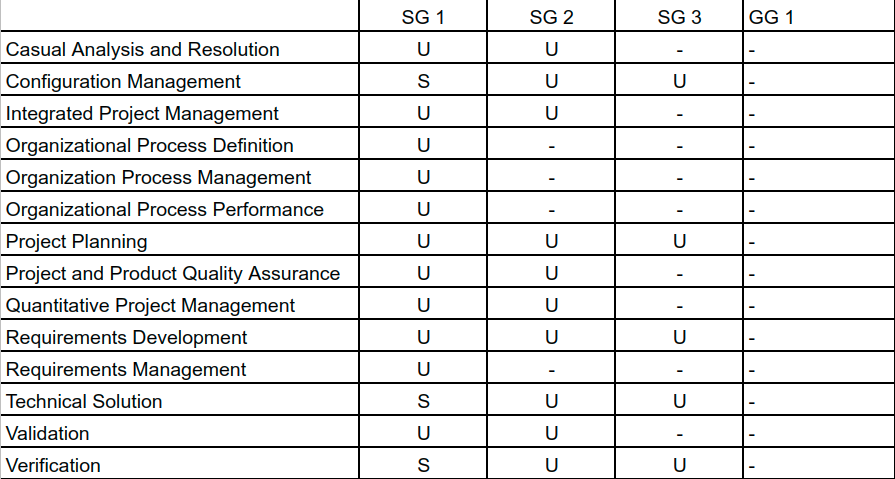
\includegraphics[scale=0.55]{img/profilisPriesLentele}
		\caption{CMMI vertinimo rezultatų gebėjimo profilis prieš pagerinimą lentelėje} % Antraštė įterpiama po paveikslėlio
		\label{img:ProfilisPries}
	\end{figure}
	\begin{figure}[!htbp]
		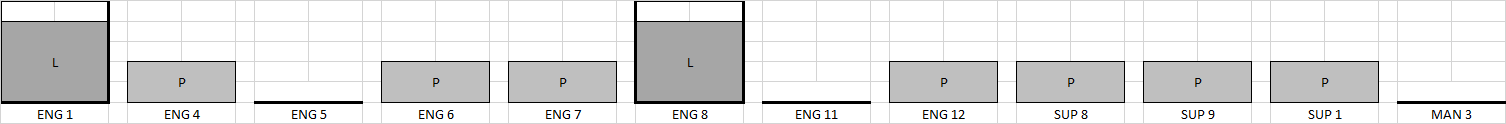
\includegraphics[scale=0.8]{img/ProfilisPries}
		\caption{CMMI vertinimo rezultatų gebėjimo profilis prieš pagerinimą} % Antraštė įterpiama po paveikslėlio
		\label{img:ProfilisPries}
	\end{figure}
	
	
	\section{Technical solution}
	
		Viena esminių produkto kūrimo procesų norint sukurti kokybišką produktą bei turėti sklandų jo kūrimo procesą yra technologinio sprendimo paieška ir įgyvendinimas, todėl ir nusprendėme patobulinti šį procesą. Jo aprašymui trūko detalumo bei praleisti svarbūs sprendimai, kuriuos reikia priimti prieš pradedant implementaciją.
		\subsection{Pagerinimas}
		\begin{itemize}
			\item{Pridėtas visų projektavimo lygių išskyrimas ir jų dokumentacijos lygio nurodymas.}
			\item{Pridėti kriterijai ir rodikliai visoms naudojamoms ir naujoms technoligijoms.}
			\item{Nustatomi sąsajų kriterijai ir sąsajos tarp komponentų ir išorės.}
			\item{Su klientu nutariama dėl alternatyvų.}
			\item{Daroma produkto perpanaudojimo analizė ir nurodomi kriterijai.}
			\item{Sukuriamas techninių duomenų paketas.}
\end{itemize}
			\subsubsection{Proceso aprašymas po pagerinimo}
			\begin{center}
		\begin{table}[ht]
			\caption{Technologinio sprendimo paieškos ir įgyvendinimo procesas.}
			\begin{tabular}{ | l | l | }
				\hline
				Pavadinimas:          & Technologinio sprendimo paieška ir įgyvendinimas.									\\ \hline
				Tikslas:              & \textcolor{black}{Išskirti technologijas ir jų versijas, kurios bus naudojamos projekte. 	}					\\ \hline
				Vykdytojai:           & \textcolor{black}{Projekto vadovas, klientas, programuotojas.}										\\ \hline
				Veiklos:              & \textcolor{blue}{V1 - Nustatomi supruojaktuojami lygiai.} 								\\
				& \textcolor{black}{V2 - Aptariamos technologijos, šiuo metu naudojamos projekte.} \\	
				& \textcolor{blue}{V3 - Nustatomi technologijų kriterijai ir rodikliai.} \\			
				& \textcolor{blue}{V4 - Nustatomi sąsajų kriterijai.} \\	
				& \textcolor{blue}{V5 - Nustomos sąsajos tarp komponentų ir su išore.} \\	
				& \textcolor{blue}{V6 - Pateikiamas palyginimas dabartinės sistemos ir kitų technologijų.} \\		
				& \textcolor{blue}{V7 - Nustatomi produkto perpanaudojimo kriterijai.} \\							
				                      & \textcolor{black}{V8 - Nustatomos technologijų kainos, kurios bus naudojamos projekte.}							\\
				                      & \textcolor{black}{V9 - Nutariama dėl technologinių alternatyvų.	}									\\ 
				                     
				& \textcolor{blue}{V10 - Kuriamas techninių duomenų paketas.} \\		\hline
				                      
				Naudojami produktai:	& \textcolor{black}{NP1 - Esamos sistemos dokumentacija, norimų naudoti technologijų} \\& \textcolor{black}{dokumentacija ir kainynas. 	}		\\ \hline
				Sukuriami produktai:	
				& \textcolor{blue}{SP1 - Technologinių duomenų paketas.}	\\
				& \textcolor{blue}{SP2 - Alternatyvių sprendimų dokumentas.}	\\\hline
			\end{tabular}
		\end{table}
	\end{center}
	\begin{enumerate}
	\item{\textcolor{blue}{Nustatomas sistemos projektavimo lygių skaičius ir kiekvienam jų tinkamas dokumentacijos lygis.}}
		\item{
			Aptariamos technologijos, kurios šiuo metu naudojamos projekte - išskiriami technologiniai karkasai, duomenų bazės, programavimo kalbų versijos ir kitos naudojamos technologijos ir jų versijos.
			Įvertinamas esamų technologijų saugumo lygis, greitaveika ir ateities palaikymas.
			Pasiūlomi technologiniai sprendimai pagrindžiant jų naudą sistemai.
		}
		\item{\textcolor{blue}{Nustatomi kriterijai, kuriuos turi įgyvendinti potencialiai nauja technologija.}}
		\item{Nustatomos technologijų kainos, kurios bus naudojamos projekte - paskaičiuojamos dabartinių technologijų kainos ir naujų siūlomų technologijų kainos.}
		\item{\textcolor{blue}{Nustatomi naudojamų ir naujų technologinių alternatyvų visi rodikliai, kokie potencialūs privalumai ir neprivalumai.}}
		\item{\textcolor{blue}{Nustatomi sąsajų kriterijai.}}
		\item{\textcolor{blue}{Nustatomos sąsajos tarp produkto komponentų bei su išoriniais objektais.}}
		\item{\textcolor{blue}{Pateikiamas palyginimai tarp dabartinės sistemos technologijos ir kitų technologijos kartu su anksčiau pateiktais kriterijais.}}
		\item{\textcolor{blue}{Nutariama dėl technologinių alternatyvų su klientu atsižvelgiant į pateiktų kriterijų įgyvendinamumą ir kainą.}}
		\item{\textcolor{blue}{Nustatomi produkto perpanaudojimo kriterijai.}}
		\item{\textcolor{blue}{Suprojektuota sistema įvertinama pagal tai, ar produkto komponentai turėtų būti sukurti, perpanaudoti ar nusipirkti.}}
		\item{\textcolor{blue}{Visi projektavimo sprendimai dokumentuojami techninių duomenų pakete.}}
	\end{enumerate}
		\subsection{NI PI LI FI atitikimas po pagerinimo}
		
		

	\section{Verification}
		Buvo nutarta, kad įmonėje vertifikaciją yra viena iš labiau išvystytų aspektų todėl norėjom jį dar labiau pastumti į priekį, kad ši sritis tarnautų dar ilgą laiką. 
		Taip pat pamanėme, kad jeigu verifikacijos veikla įmonėje būtų išvystyta pilniau, būtų mažiau pataisymų, perdarimų ir konfliktų su užsakovų dėl produkto kuris neatitiktų reikalavimų.
		\subsection{Pagerinimas}
			\begin{itemize}
				\item{Sukurtas kolegų peržvalgos procesas.}
				\item{Patobulintas kokybės užtikrinimol procesas, pridėta veiklų.}
				\item{Padidintas sukūriamos dokumentacijos kiekis.}
			\end{itemize}
			\subsubsection{Proceso aprašymas po pagerinimo}
				\begin{figure}[!htbp]
					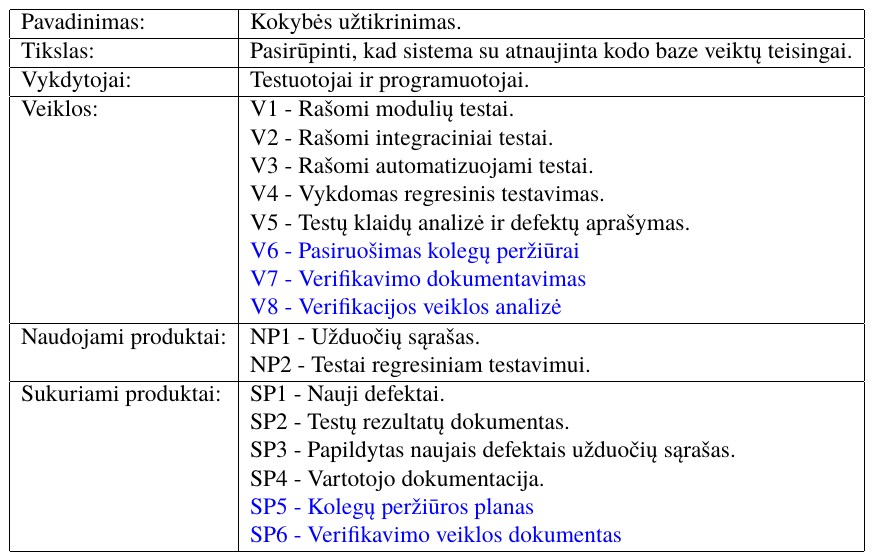
\includegraphics[scale=0.8]{img/kokybepo}
					\caption{Kokybės užtikrinimo procesas po patobulinimo} % Antraštė įterpiama po paveikslėlio
					\label{img:ProfilisPo}
				\end{figure}

\pagebreak

				\begin{figure}[!htbp]
					
\includegraphics[scale=0.8]{img/kokybepotwo}
					\caption{Kokybės užtikrinimo procesas po patobulinimo} % Antraštė įterpiama po paveikslėlio
					\label{img:ProfilisPo}
				\end{figure}
				\begin{figure}[!htbp]
					
\includegraphics[scale=0.8]{img/kokybepothree}
					\caption{Kokybės užtikrinimo procesas po patobulinimo} % Antraštė įterpiama po paveikslėlio
					\label{img:ProfilisPo}
				\end{figure}

\pagebreak

				\begin{figure}[!htbp]
					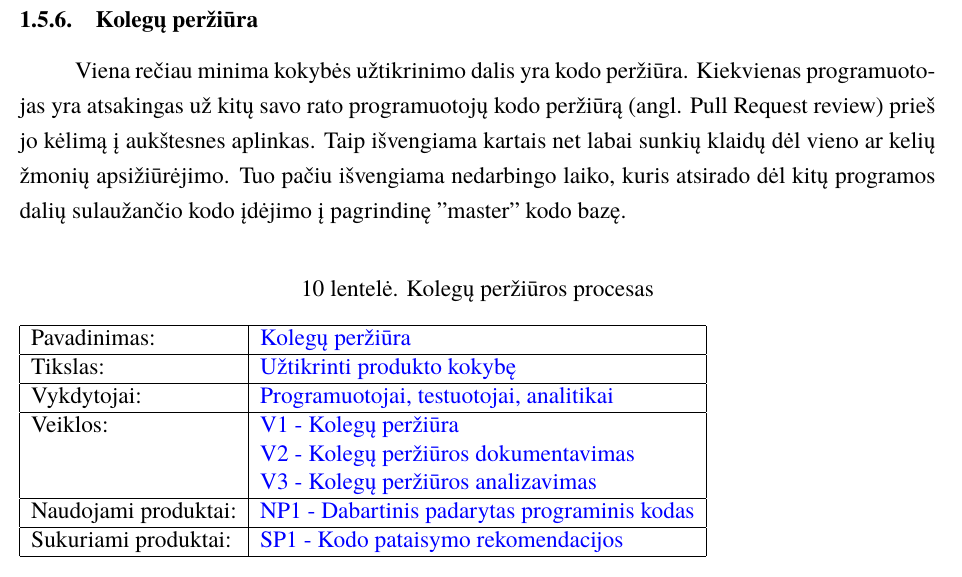
\includegraphics[scale=0.8]{img/kolegupoone}
					\caption{Kolegų peržiūros procesas} % Antraštė įterpiama po paveikslėlio
					\label{img:ProfilisPo}
				\end{figure}
				\begin{figure}[!htbp]
					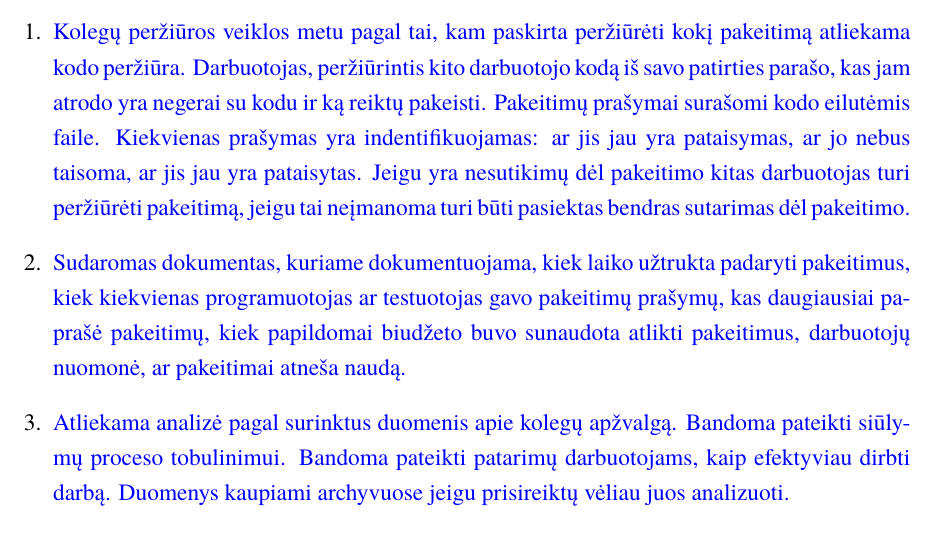
\includegraphics[scale=0.8]{img/kolegupotwo}
					\caption{Kolegų peržiūros procesas} % Antraštė įterpiama po paveikslėlio
					\label{img:ProfilisPo}
				\end{figure}

		\subsection{NI PI LI FI atitikimas po pagerinimo}
\pagebreak
				\begin{figure}[!htbp]
					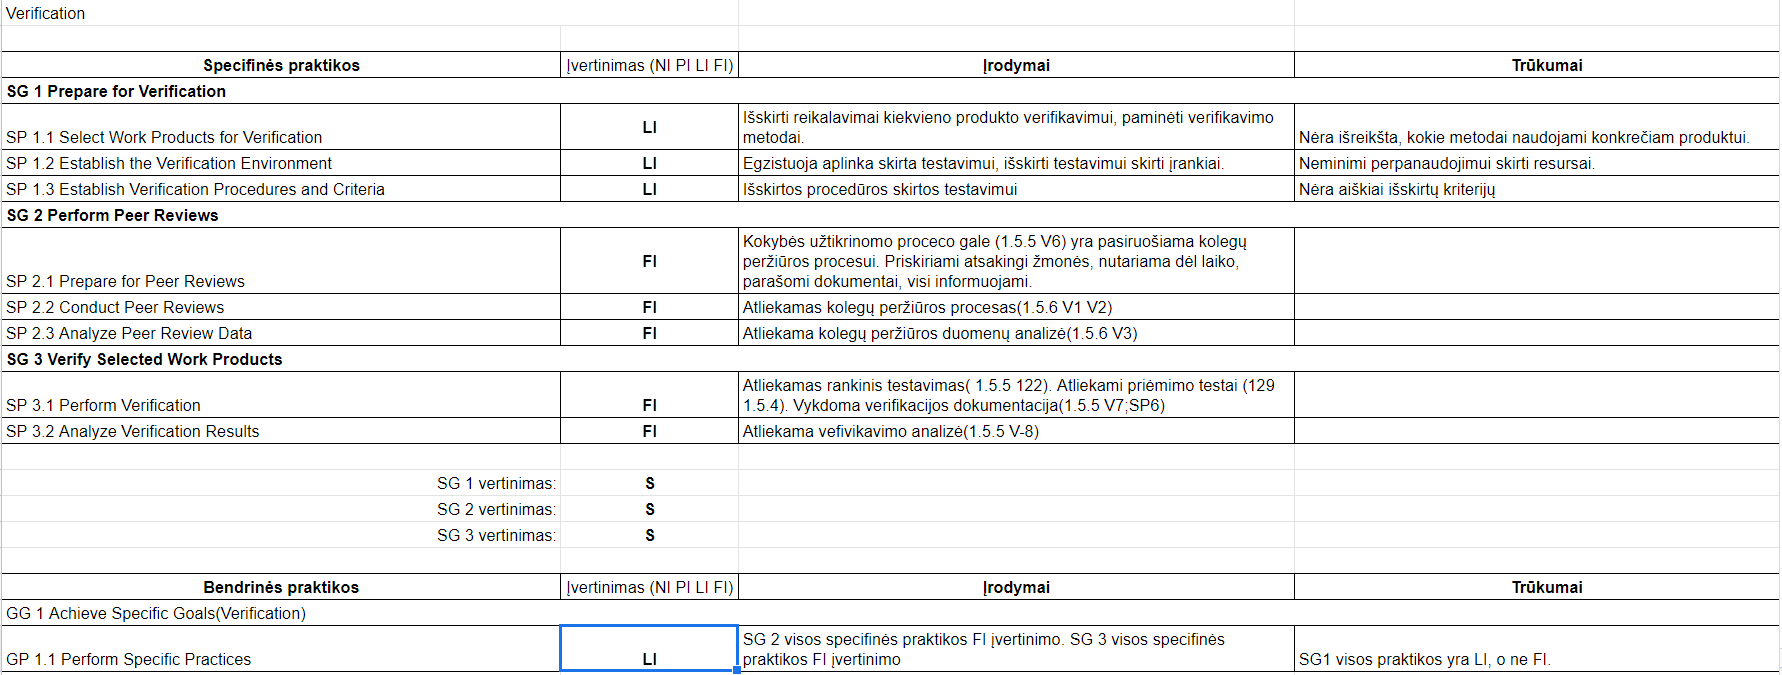
\includegraphics[scale=0.4]{img/verfpo}
					\caption{Verifikavimo vertinimas po patobulinimo} % Antraštė įterpiama po paveikslėlio
					\label{img:ProfilisPo}
				\end{figure}
	\section{Configuration management}
	Konfigūracijos valdymas yra vienas svarbiausių procesų norint patikimai kurti programų sistemas, todėl pasirinkome jį tobulinti.
		\subsection{Pagerinimas}
		\begin{itemize}
			\item Pridėtos veiklos standarto išleidimui, pakeitimų dokumentavimui bei auditui.
			\item Pridėtas konfigūracijos pakeitimų prioritizavimas.
		\end{itemize}
			\subsubsection{Proceso aprašymas po pagerinimo}
			\begin{center}
				\begin{table}[ht]
					\caption{Konfigūracijos valdymo procesas}
					\begin{tabular}{ | l | l | }
						\hline
						Pavadinimas:         & Konfigūracijos valdymas.				\\ \hline
						Tikslas:             & \textcolor{black}{Atnaujinti sprinto konfigūraciją.}			\\ \hline
						Vykdytojai:          & \textcolor{black}{devOps specialistai, programuotojai.}			\\ \hline
						Veiklos:             	& \textcolor{blue}{V1 - Pakeitimų validumo užtikrinimas.	}		\\ \hline
																& \textcolor{black}{V2 - Repozitorijos su konfigūracijomis atnaujinimas.}	\\
																 & \textcolor{black}{V3 - Duomenų bazės atnaujinimas.	}		\\ \hline
																 & \textcolor{blue}{V4 - Standarto išleidimas.	}		\\ \hline
																 & \textcolor{blue}{V5 - Konfigūracinių pakeitimų dokumentavimas.	}		\\ \hline
																 & \textcolor{blue}{V6 - Konfigūracijos pakeitimų auditas.	}		\\ \hline
						Naudojami produktai: & \textcolor{black}{NP1 - Konfigūracijos pakeitimų sąrašas.	}	\\ \hline
						Sukuriami produktai: & \textcolor{black}{SP1 - Pamodifikuota konfigūracijų repozitorija. }	\\
																 & \textcolor{black}{SP2 - Atnaujinta duomenų bazė. }			\\ \hline
																 & \textcolor{blue}{SP3 - Konfigūracijos standarto dokumentas. }			\\ \hline
																 & \textcolor{blue}{SP3 - Audito rezultatų dokumentas. }			\\ \hline
																 & \textcolor{blue}{SP4 - Konfigūracinių pakeitimų dokumentas. }			\\ \hline
					\end{tabular}
				\end{table}
			\end{center}
				\textcolor{blue}{Sprinto metu atlikti konfigūracijos pakeitimai yra prioritizuojami pagal jų svarbą, patikrinimas jų validumas, ar jie yra autorizuoti.}\textcolor{black}{Sprinto pabaigoje devOps specialistai peržvelgia atliktus konfigūracinius pakeitimus, kuriuos programuotojai pažymi sprinto metu.
				Šie konfigūracijos pakeitimai yra įdedami į aukštesnę aplinką.} Taip pat po sprinto kodas yra sudedamas į aukštesnę aplinką tolimesniam testavimui.
				\textcolor{blue}{Pagal skirtingus kvalifikacijos lygius programuotojams ar kitiems specialistams suteikiami skirtingi leidimai peržiūrėti/keisti konfigūracijas. Atlikus konfigūracinius pakeitimus sukuriamas dokumentas su konfigūracijos metrikomis, pagal kurį būtų galima atkurti esamą sistemos būseną. Šiam dokumentui priskiriamas unikalus numeris.} \newline
				\textcolor{blue}{Atlikti konfigūraciniai pakeitimai yra detaliai dokumentuojami, yra užtikrinama, kad reikiami asmenys turėtų prieigą prie šių pakeitimų būsenos.} \newline
				\textcolor{blue}{Konfigūracijos pakeitimai taip pat sudedami į tam skirtą duomenų bazę tolimesniam jų sekimui.} \newline
				\textcolor{blue}{Po visų pakeitmų atliekamas auditas norint užtikrinti, ar naujai išleistas standartas yra integralus, ar konfigūraciniai įrašai atitinka konfigūracinius vienetus. Patvirtinamas konfigūracinių vienetų pilnumas, jų nuoseklumas. Radus neatitikimų sukuriamas veiksmų planas jiems išspręsti.}
		\subsection{NI PI LI FI atitikimas po pagerinimo}
		\begin{figure}[!htbp]
			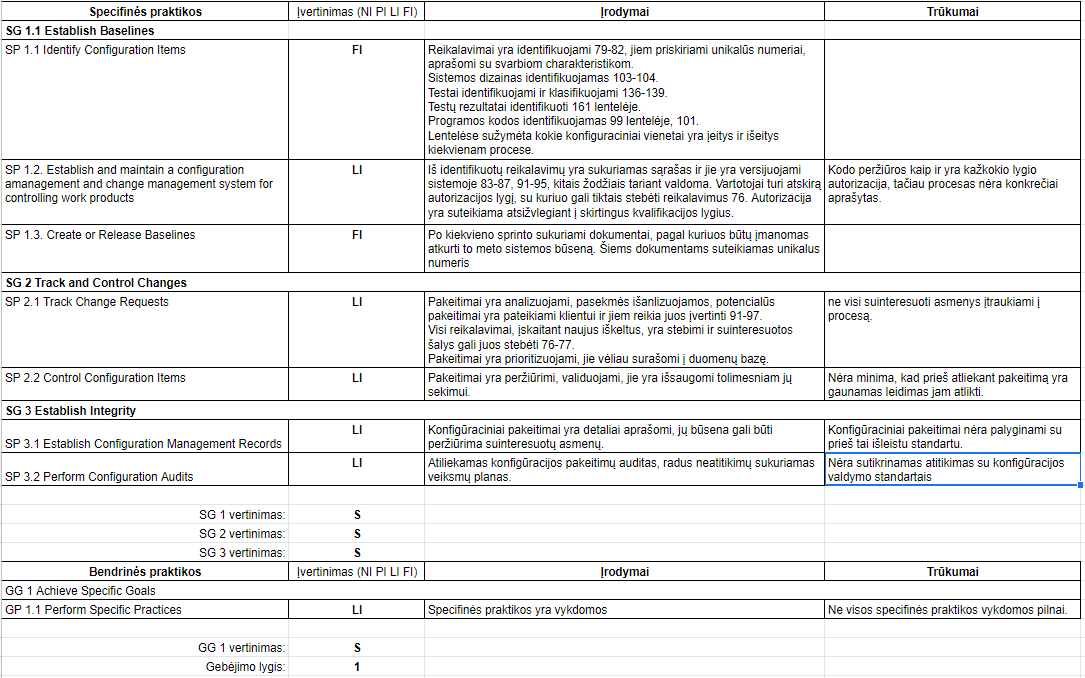
\includegraphics[scale=0.6]{img/konfiguracijosValdymasPataisytas}
			\caption{Konfigūracijos valdymo vertimas po pataisymo} % Antraštė įterpiama po paveikslėlio
			\label{img:ProfilisPo}
		\end{figure}
	\section{Vertinimo rezultatai po pagerinimo}
	\begin{figure}[!htbp]
		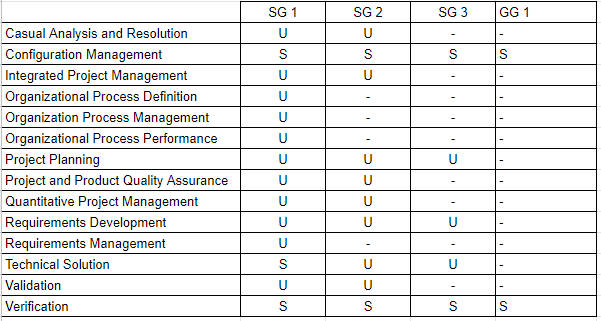
\includegraphics[scale=0.9]{img/poPataisymo}
		\caption{CMMI vertinimo rezultatų gebėjimo profilis po pagerinimo lentelėje} % Antraštė įterpiama po paveikslėlio
		\label{img:ProfilisPo}
	\end{figure}
	\begin{figure}[!htbp]
		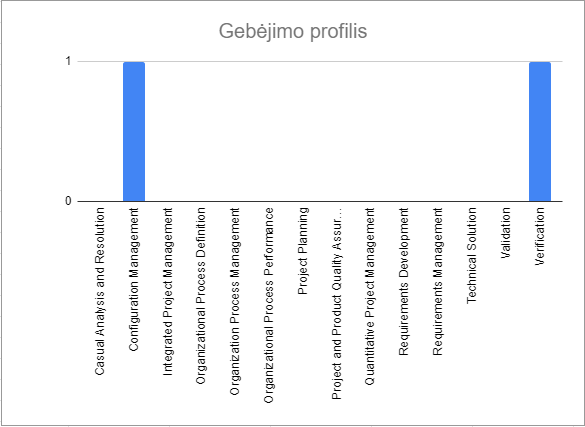
\includegraphics[scale=0.8]{img/poPataisymoProfilis}
		\caption{CMMI vertinimo rezultatų gebėjimo profilis po pagerinimo} % Antraštė įterpiama po paveikslėlio
		\label{img:ProfilisPo}
	\end{figure}
\section{Rezultatai ir išvados}
Po procesų pagerinimo pavyko sėkmingai pakelti du procesus iki pilno pirmo CMMI brandos
lygio. Išsiaiškinom ir supratom, kad net ir nedideli bet tikslingi pakeitimai procese padaro daug
teigiamos įtakos kokybei.
\end{document}
